%% -----------------------------------------------------------------------------

\chapter{Background}\label{ch:background}

Background information on technologies used.


\section{Memory Safety and Layout}

General stack layout, buffer overflow description, common pitfalls especially in systems languages

\begin{figure}[htp!]
%\vspace{2mm}
\centering
    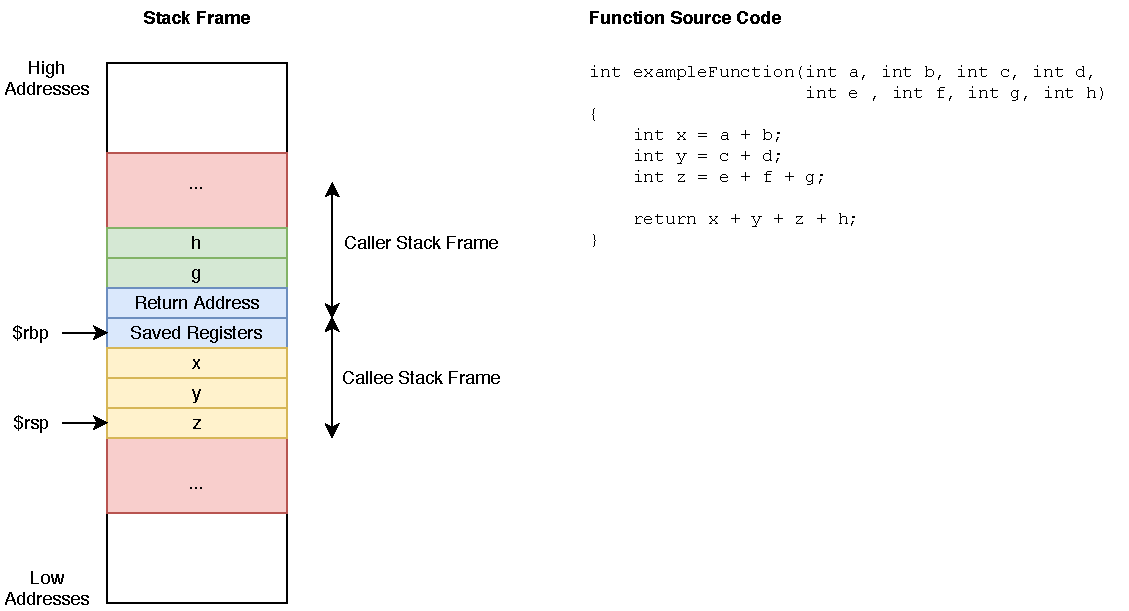
\includegraphics[width=\textwidth]{assets/figures/chapter2/frame.pdf}
    \caption{Stack Frame Layout}
    \label{fig:stack-frame-layout}
    %\vspace{-10pt}
\end{figure}

\begin{figure}[htp!]
    %\vspace{2mm}
    \centering
    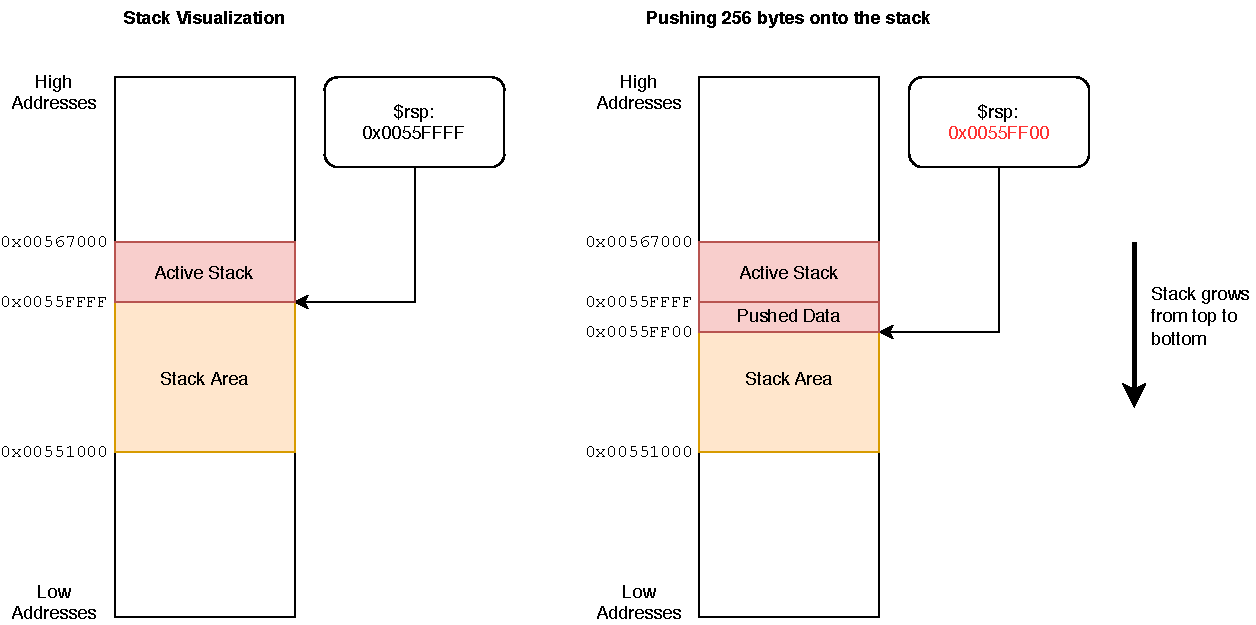
\includegraphics[width=\textwidth]{assets/figures/stack.pdf}
    \caption{Pushing to the Stack}
    \label{fig:stack}
    %\vspace{-10pt}
\end{figure}


Systems languages have many pitfalls: buffer overflows, use-after-frees, heap overflows, ...

Huge security implications, tons of bugs especially with cryptographic C code that gets
used in the internet.

Compiler features to statically prove upon compilation that a program does not contain any
buffer overflows etc.

Usually more verbose programming style, but enables to automatically check the program
on security vulnerabilities.

How is it syntactically achieved in Go?


\section{Go Unsafe API}

Introduction into the unsafe package, what operations exist?

Sometimes the programmer might need to bypass the safe guards, e.g. for optimizations or
interoperability with native unsafe code, that is C libraries.

Explain language features to achieve unsafe code. How does such code look like?

In the case of Go there are unsafe pointers from the unsafe package. Explain how they
can be used, and which reasons there might be to use some.


\section{Dependency Management}

Developers should not reinvent the wheel, instead they should make use of dependencies.

Code is imported into a project. The code is reused, but the project of course also inherits
all security vulnerabilities of the dependencies.

How are Go modules organized? How is the Go.mod file written? How is code imported?

Since lots of projects use the same dependencies, we can link projects in a dependency
graph that shows usage of libraries in the software landscape.

Especially open source software makes it easy to analyze the dependency graph, and with
open source it is very important to reuse dependencies because time is valuable and a lot
of open source projects are non-profit.
